\documentclass{article}
\usepackage{amsmath,amssymb,amsthm,latexsym,paralist,relsize}
\usepackage{graphicx}
\usepackage[margin=1.5in]{geometry}
\usepackage{titling}
\usepackage{xcolor}
\usepackage{float}
\usepackage{enumitem}
\usepackage{caption}
\usepackage{subcaption}
\setlength{\droptitle}{-10em}   % This is your set screw
\DeclareRobustCommand{\stirling}{\genfrac\{\}{0pt}{}}
\theoremstyle{definition}

%\newtheorem{definition}{Definition}
%\newtheorem{proof}{Proof}
%\newtheorem{remark}{Remark}


\newtheorem{problem}{Problem}
\newtheorem*{solution}{Solution}
\newtheorem*{resources}{Resources}


% Self Explanatory
\newtheorem{theorem}{Theorem}[section]
\newtheorem{definition}{Definition}
\newtheorem{corollary}{Corollary}[theorem]

\newtheorem{example}{Example}

\newtheorem{lemma}[theorem]{Lemma}


\newcommand{\ep}{\varepsilon}
\newcommand{\vp}{\varphi}
\newcommand{\lam}{\lambda}
\newcommand{\Lam}{\Lambda}
%\newcommand{\abs}[1]{\ensuremath{\left\lvert#1\right\rvert}} % This clashes with the physics package
%\newcommand{\norm}[1]{\ensuremath{\left\lVert#1\right\rVert}} % This clashes with the physics package

\newcommand{\floor}[1]{\ensuremath{\left\lfloor#1\right\rfloor}}
\newcommand{\ceil}[1]{\ensuremath{\left\lceil#1\right\rceil}}
\newcommand{\A}{\mathbb{A}}
\newcommand{\B}{\mathbb{B}}
\newcommand{\C}{\mathbb{C}}
\newcommand{\D}{\mathbb{D}}
\newcommand{\E}{\mathbb{E}}
\newcommand{\F}{\mathbb{F}}
\newcommand{\K}{\mathbb{K}}
\newcommand{\N}{\mathbb{N}}
\newcommand{\Q}{\mathbb{Q}}
\newcommand{\R}{\mathbb{R}}
\newcommand{\T}{\mathbb{T}}
\newcommand{\X}{\mathbb{X}}
\newcommand{\Y}{\mathbb{Y}}
\newcommand{\Z}{\mathbb{Z}}
\newcommand{\As}{\mathcal{A}}
\newcommand{\Bs}{\mathcal{B}}
\newcommand{\Cs}{\mathcal{C}}
\newcommand{\Ds}{\mathcal{D}}
\newcommand{\Es}{\mathcal{E}}
\newcommand{\Fs}{\mathcal{F}}
\newcommand{\Gs}{\mathcal{G}}
\newcommand{\Hs}{\mathcal{H}}
\newcommand{\Is}{\mathcal{I}}
\newcommand{\Js}{\mathcal{J}}
\newcommand{\Ks}{\mathcal{K}}
\newcommand{\Ls}{\mathcal{L}}
\newcommand{\Ms}{\mathcal{M}}
\newcommand{\Ns}{\mathcal{N}}
\newcommand{\Os}{\mathcal{O}}
\newcommand{\Ps}{\mathcal{P}}
\newcommand{\Qs}{\mathcal{Q}}
\newcommand{\Rs}{\mathcal{R}}
\newcommand{\Ss}{\mathcal{S}}
\newcommand{\Ts}{\mathcal{T}}
\newcommand{\Us}{\mathcal{U}}
\newcommand{\Vs}{\mathcal{V}}
\newcommand{\Ws}{\mathcal{W}}
\newcommand{\Xs}{\mathcal{X}}
\newcommand{\Ys}{\mathcal{Y}}
\newcommand{\Zs}{\mathcal{Z}}
\newcommand{\ab}{\textbf{a}}
\newcommand{\bb}{\textbf{b}}
\newcommand{\cb}{\textbf{c}}
\newcommand{\db}{\textbf{d}}
\newcommand{\ub}{\textbf{u}}
%\renewcommand{\vb}{\textbf{v}} % This clashes with the physics package (the physics package already defines the \vb command)
\newcommand{\wb}{\textbf{w}}
\newcommand{\xb}{\textbf{x}}
\newcommand{\yb}{\textbf{y}}
\newcommand{\zb}{\textbf{z}}
\newcommand{\Ab}{\textbf{A}}
\newcommand{\Bb}{\textbf{B}}
\newcommand{\Cb}{\textbf{C}}
\newcommand{\Db}{\textbf{D}}
\newcommand{\eb}{\textbf{e}}
\newcommand{\ex}{\textbf{e}_x}
\newcommand{\ey}{\textbf{e}_y}
\newcommand{\ez}{\textbf{e}_z}
\newcommand{\abar}{\overline{a}}
\newcommand{\bbar}{\overline{b}}
\newcommand{\cbar}{\overline{c}}
\newcommand{\dbar}{\overline{d}}
\newcommand{\ubar}{\overline{u}}
\newcommand{\vbar}{\overline{v}}
\newcommand{\wbar}{\overline{w}}
\newcommand{\xbar}{\overline{x}}
\newcommand{\ybar}{\overline{y}}
\newcommand{\zbar}{\overline{z}}
\newcommand{\Abar}{\overline{A}}
\newcommand{\Bbar}{\overline{B}}
\newcommand{\Cbar}{\overline{C}}
\newcommand{\Dbar}{\overline{D}}
\newcommand{\Ubar}{\overline{U}}
\newcommand{\Vbar}{\overline{V}}
\newcommand{\Wbar}{\overline{W}}
\newcommand{\Xbar}{\overline{X}}
% \newcommand{\ybar}{\overline{y}}
\newcommand{\Zbar}{\overline{Z}}
\newcommand{\Aint}{A^\circ}
\newcommand{\Bint}{B^\circ}
\newcommand{\limk}{\lim_{k\to\infty}}
\newcommand{\limm}{\lim_{m\to\infty}}
\newcommand{\limn}{\lim_{n\to\infty}}
\newcommand{\limx}[1][a]{\lim_{x\to#1}}
\newcommand{\liminfm}{\liminf_{m\to\infty}}
\newcommand{\limsupm}{\limsup_{m\to\infty}}
\newcommand{\liminfn}{\liminf_{n\to\infty}}
\newcommand{\limsupn}{\limsup_{n\to\infty}}
\newcommand{\sumkn}{\sum_{k=1}^n}
\newcommand{\sumin}{\sum_{i=1}^n}
\newcommand{\sumk}[1][1]{\sum_{k=#1}^\infty}
\newcommand{\summ}[1][1]{\sum_{m=#1}^\infty}
\newcommand{\sumn}[1][1]{\sum_{n=#1}^\infty}
\newcommand{\emp}{\varnothing}
\newcommand{\exc}{\backslash}
\newcommand{\sub}{\subseteq}
\newcommand{\sups}{\supseteq}
\newcommand{\capp}{\bigcap}
\newcommand{\cupp}{\bigcup}
\newcommand{\kupp}{\bigsqcup}
\newcommand{\cappkn}{\bigcap_{k=1}^n}
\newcommand{\cuppkn}{\bigcup_{k=1}^n}
\newcommand{\kuppkn}{\bigsqcup_{k=1}^n}
\newcommand{\cappk}[1][1]{\bigcap_{k=#1}^\infty}
\newcommand{\cuppk}[1][1]{\bigcup_{k=#1}^\infty}
\newcommand{\cappm}[1][1]{\bigcap_{m=#1}^\infty}
\newcommand{\cuppm}[1][1]{\bigcup_{m=#1}^\infty}
\newcommand{\cappn}[1][1]{\bigcap_{n=#1}^\infty}
\newcommand{\cuppn}[1][1]{\bigcup_{n=#1}^\infty}
\newcommand{\kuppk}[1][1]{\bigsqcup_{k=#1}^\infty}
\newcommand{\kuppm}[1][1]{\bigsqcup_{m=#1}^\infty}
\newcommand{\kuppn}[1][1]{\bigsqcup_{n=#1}^\infty}
\newcommand{\cappa}{\bigcap_{\alpha\in I}}
\newcommand{\cuppa}{\bigcup_{\alpha\in I}}
\newcommand{\kuppa}{\bigsqcup_{\alpha\in I}}
\newcommand{\Rx}{\overline{\mathbb{R}}}
\newcommand{\dx}{\,dx}
\newcommand{\dy}{\,dy}
\newcommand{\dt}{\,dt}
\newcommand{\dax}{\,d\alpha(x)}
\newcommand{\dbx}{\,d\beta(x)}
\DeclareMathOperator{\glb}{\text{glb}}
\DeclareMathOperator{\lub}{\text{lub}}
\newcommand{\xh}{\widehat{x}}
\newcommand{\yh}{\widehat{y}}
\newcommand{\zh}{\widehat{z}}
\newcommand{\<}{\langle}
\renewcommand{\>}{\rangle}
\renewcommand{\iff}{\Leftrightarrow}
\DeclareMathOperator{\im}{\text{im}}
\let\spn\relax\let\Re\relax\let\Im\relax
\DeclareMathOperator{\spn}{\text{span}}
\DeclareMathOperator{\Re}{\text{Re}}
\DeclareMathOperator{\Im}{\text{Im}}
\DeclareMathOperator{\diag}{\text{diag}}

\newcommand{\RN}[1]{%
  \textup{\uppercase\expandafter{\romannumeral#1}}%
}

\newcommand\defeq{\mathrel{\overset{\makebox[0pt]{\mbox{\normalfont\tiny\sffamily def}}}{=}}}

\newcommand{\bhat}{\hat{\beta_1}}

% Typed name, course, email address
\title{CSCE 420 : HW 4}
\author{William Allen}
\date{\today}

\begin{document}
\maketitle


\begin{enumerate}[label=\textbf{\Alph*}]
  %% MAJOR PROBLEM  
  \item Bayesian Inference


  \vspace{1.5em}
    Consider two factors that influence whether a student passes a given test: a) being smart, and b) studying. Suppose 30\% of students believe they are intrinsically smart. But since students do not know a priori whether they are smart enough to pass a test, suppose 40\% of will study for it anyway. (assume Smart and Study are independent). The causal relationship of these variables on the probability of actually passing the test can be expressed in a conditional probability table (CPT) as follows:
    
    \begin{table}[h!]
    \centering
    \begin{tabular}{|l|l|l|}
    \hline
    P(pass$|$Smart, Study) & $\neg$smart & smart \\ \hline
    $\neg$study          & 0.2         & 0.7   \\ \hline
    study                & 0.6         & 0.95  \\ \hline
    \end{tabular}
    \end{table}

    prior probabilities: P(smart)=0.3, P(study)=0.4

    \begin{enumerate}[label=(\alph*)]
        \item Write out the equation for calculating joint probabilities, P(Smart,Study,Pass).
        \item Calculate all the entries in the full joint probability table (JPT) [a 4x2 matrix, like Fig 12.3 in the textbook; [Note: names of variables are capitalized, lower-case indicates truth value, e.g. ‘pass’ means Pass=T, and ‘-pass’ means Pass=F.]
        \item From the JPT, compute the probability that a student is smart, given that they pass the test but did not study.
        \item From the JPT, compute the probability that a student did not study, given that they are smart but did not pass the test.
        \item Compute the marginal probability that a student will pass the test given that they are smart.
        \item Compute the marginal probability that a student will pass the test given that they study.
    \end{enumerate}
      %% SOLUTION
      \vspace{1em} 
      \textit{ Sol. }
      \vspace{1em}
      \begin{quote}
        \begin{enumerate}[label=(\alph*)]
        \item The equation for calculating joint probabilities, P(Smart,Study,Pass) is:
        \begin{align*}
          P(Smart, Study, Pass) &= P(Pass \mid Smart, Study) \cdot P(Smart) \cdot P(Study)
        \end{align*}
        \item 
            \begin{table}[h!]
            \centering
            \begin{tabular}{|c|c|c|c|}
            \hline
            \textbf{Smart} & \textbf{Study} & \textbf{Pass = False} & \textbf{Pass = True} \\
            \hline
            False & False & 0.336 & 0.084 \\
            \hline
            False & True & 0.112 & 0.168 \\
            \hline
            True & False & 0.054 & 0.126 \\
            \hline
            True & True & 0.006 & 0.114 \\
            \hline
            \end{tabular}
            \end{table}
    
        \item We will use the Bayes' theorem:
        \begin{align*}
            P(smart \mid pass, -study) &= \frac{P(pass, -study \mid smart) \cdot P(smart)}{P(pass, -study)}\\
            &= \frac{P(smart, -study, pass)}{P(smart, -study, pass) + P(-smart, -study, pass)}\\
            &= \frac{0.126}{0.126 + 0.084} = 0.6
        \end{align*}
        
        \item From the JPT,
        \begin{align*}
            P(-study \mid smart, -pass) &= \frac{P(smart, -pass \mid -study) \cdot P(-study)}{P(smart, -pass)}\\
            &= \frac{P(smart, -study, -pass)}{P(smart, study, -pass) + P(smart, -study, -pass)}\\
            &= \frac{0.054}{0.006 + 0.054} = 0.9
        \end{align*}
        
        \item To compute the marginal probability that a student will pass the test given that they are smart, we sum over all possible values of Study:
        \begin{align*}
            P(pass \mid smart) &= \sum_{study}P(smart, study, pass)\\
            &= P(smart, study, pass) + P(smart, -study, pass)\\
            &= 0.114 + 0.126 = 0.24
        \end{align*}
        
        \item To compute the marginal probability that a student will pass the test given that they study, we sum over all possible values of Smart:
        \begin{align*}
            P(pass \mid study) &= \sum_{smart}P(smart, study, pass)\\
            &= P(smart, study, pass) + P(-smart, study, pass)\\
            &= 0.114 + 0.168 = 0.282
        \end{align*}
        \end{enumerate}
      \end{quote}

%% MAJOR PROBLEM
\item 2. Bayesian Networks. 

  \vspace{1.5em}
  Here is a probabilistic model that describes what it might mean when a person sneezes, e.g. depending on whether they have a cold, or whether a cat is present and they are allergic. Scratches on the furniture would be evidence that a cat had been present.

    \begin{figure}[h!]
        \centering
        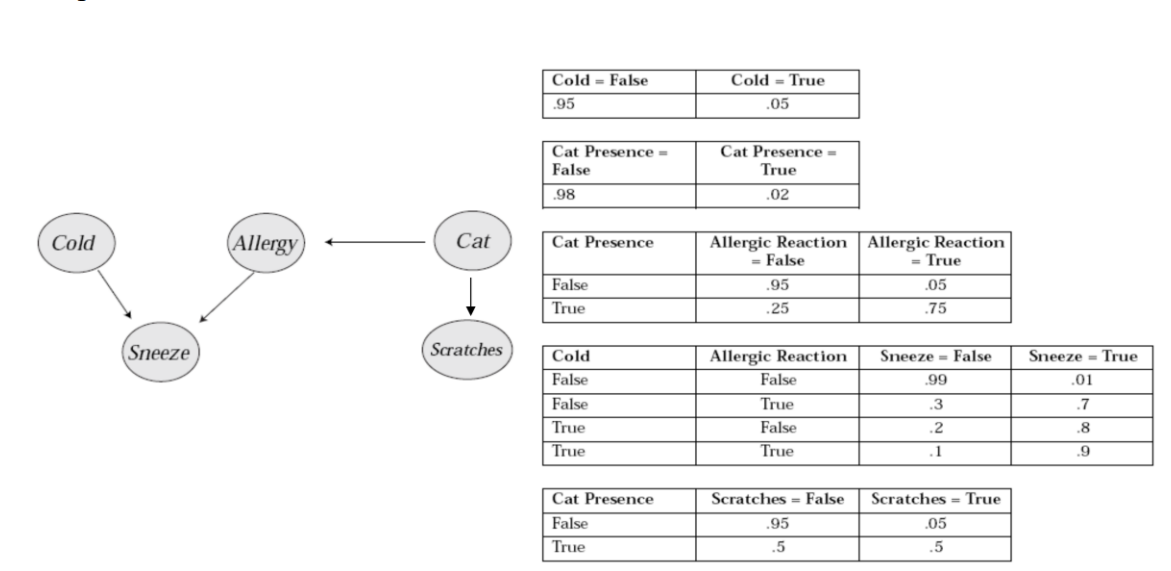
\includegraphics{fig1.PNG}
        \caption{Caption}
        \label{fig:my_label}
    \end{figure}

    a) Using Equation 13.2 in the textbook (p. 415), write out the expression for the joint probability for any state (combination of truth values for the 5 variables). [Note: Use capital letters for names of variables, and lower-case to indicate truth value, e.g. ‘cold’ means Cold=T, and ‘-cold’ means Cold=F.]

    b) Use the joint prob. equation to calculate the probability for all 32 entries in the JPT. (you might want to write a little script to do this)

    c) Calculate the probability that someone is allergic, given that they sneezed but do not have a cold, and it is unknown whether a cat has been present but there are scratches on the furniture, $P(allergic \mid sneeze,\neg cold,scratches)$. Do this calculation numerically using entries in the JPT. (hint: you will have to marginalize over cat presence.)


      %% SOLUTION
      \vspace{1em} 
      \textit{ Sol. }
      \begin{quote}
        a) $P(Cold, Cat, Allergy, Sneeze, Scratches) = P(Cold) \cdot P(Cat) \cdot P(Allergy \mid Cat) \cdot P(Sneeze \mid Cold, Allergy) \cdot P(Scratches \mid Cat)$ 
        \newpage
        b)
        \begin{table}[h ]
        \centering
        \begin{tabular}{|c|c|c|c|c|c|}
        \hline
        Cold & Allergy & Cat & Sneeze & Scratches & Joint Probability \\ \hline
        False & False & False & False & False & 0.83183 \\ \hline
        False & False & False & False & True & 0.04378 \\ \hline
        False & False & False & True & False & 0.00840 \\ \hline
        False & False & False & True & True & 0.00044 \\ \hline
        False & False & True & False & False & 0.00235 \\ \hline
        False & False & True & False & True & 0.00235 \\ \hline
        False & False & True & True & False & 0.00002 \\ \hline
        False & False & True & True & True & 0.00002 \\ \hline
        False & True & False & False & False & 0.01327 \\ \hline
        False & True & False & False & True & 0.00070 \\ \hline
        False & True & False & True & False & 0.03096 \\ \hline
        False & True & False & True & True & 0.00163 \\ \hline
        False & True & True & False & False & 0.00214 \\ \hline
        False & True & True & False & True & 0.00214 \\ \hline
        False & True & True & True & False & 0.00499 \\ \hline
        False & True & True & True & True & 0.00499 \\ \hline
        True & False & False & False & False & 0.00884 \\ \hline
        True & False & False & False & True & 0.00047 \\ \hline
        True & False & False & True & False & 0.03538 \\ \hline
        True & False & False & True & True & 0.00186 \\ \hline
        True & False & True & False & False & 0.00003 \\ \hline
        True & False & True & False & True & 0.00003 \\ \hline
        True & False & True & True & False & 0.00010 \\ \hline
        True & False & True & True & True & 0.00010 \\ \hline
        True & True & False & False & False & 0.00023 \\ \hline
        True & True & False & False & True & 0.00001 \\ \hline
        True & True & False & True & False & 0.00209 \\ \hline
        True & True & False & True & True & 0.00011 \\ \hline
        True & True & True & False & False & 0.00004 \\ \hline
        True & True & True & False & True & 0.00004 \\ \hline
        True & True & True & True & False & 0.00034 \\ \hline
        True & True & True & True & True & 0.00034 \\ \hline
        \end{tabular}
        \end{table}
        \newpage
        c) We can use the formula: 
        First, we need to find the joint probability for the given conditions:
        \begin{equation*}
        P(allergic, sneeze, \neg cold, scratches) = \sum_{cat} P(\neg cold, cat, allergic, sneeze, scratches)
        \end{equation*}
        From the table, this is equal to 0.00163 + 0.00499 = 0.00662.
        
        Next, we need to calculate the marginal probability for the given evidence:
        
        \begin{equation*}
        P(sneeze, \neg cold, scratches) = \sum_{cat, allergic} P(\neg cold, cat, allergic, sneeze, scratches)
        \end{equation*}
        From the table, this is equal to 0.00044 + 0.00002 + 0.00163 + 0.00499 = 0.00708.
        
        Therefore, we get $P(allergic | sneeze, ¬cold, scratches)$ = 0.00662 / 0.00708 = 0.935.
    \end{quote}

\newpage

%% MAJOR PROBLEM
\item PDDL and Situation Calculus

  \vspace{1.5em}
  
    Starting a car: You have to be at the car and have the key, and the car has to have a charged battery and the tank has to have gas. Afterwards, the car will be running, and you will still be at the car and have the key after starting the engine. 

    a. Write a PDDL operator to describe this action.
(note: you can express this ego-centrically – you don’t have to refer explicitly to the
person starting the car; but the operator should take the car being started as an argument)

    b. Describe the same operator using Situation Calculus (remember to add a situation
argument to your predicates).

    c. Add a Frame Axiom that says that starting this car will not changes whether any other
car is out of gas (tank empty).
    %% SOLUTION
    \vspace{1em} 
    
    \textit{ Sol. }
    \begin{quote}
        a. startCar(car):
        \begin{itemize}
            \item  pre-conds: atCar(), hasKey(), chargedBattery(car), hasGas(car)
            \item effects: carRunning(car), atCar(), hasKey()
        \end{itemize}
        b. \\
        $\forall s$ Poss(startCar(car), s) $\iff$ (Holds(AtCar(), s) $\land$ Holds(HasKey(), s) $\land$ Holds(ChargedBattery(car), s) $\land$ Holds(HasGas(car), s)) \\ \\
        $\forall s$ Holds(CarRunning(car), do(startCar(car), s)) $\iff$ (Holds(AtCar(), s) $\land$ Holds(HasKey(), s) $\land$ Holds(ChargedBattery(car), s) $\land$ Holds(HasGas(car), s))
    
        c. $\forall$ car1, car2, s (car1 ≠ car2) → (Holds(OutOfGas(car1), do(startCar(car2), s)) $\iff$ Holds(OutOfGas(car1), s))
    \end{quote}
    
\end{enumerate}
\end{document}
